\section{開発の背景}
近年,ナレッジマネジメントが企業経営の重要な要素と言われ,導入する企業が増えている.
ナレッジマネジメントとは,個人の持つ知識や情報を組織全体で共有し,
有効に活用することで業績を上げようという経営手法である.
日本語では,「知識管理」などと訳され,「KM」と略されることもある\cite{a}.

ナレッジマネジメントでは,グループ開発において共有する知識は
暗黙知と形式知に分けられる\cite{b}.
暗黙知は主に口伝によって一対一でつたえられたり,あるいは体で覚えるというのが一般的である.
しかし,定着するまでの間は一般的にメモという形で個人的な知識として扱われるのが普通である.
一方で図書館やwebなどでは文書やhyper textとして誰もが読める形で保管,提供される知識は形式知と呼ばれる.図\ref{knowledge}に暗黙知と形式知をまとめた.


\begin{figure}[htbp]
\begin{center}
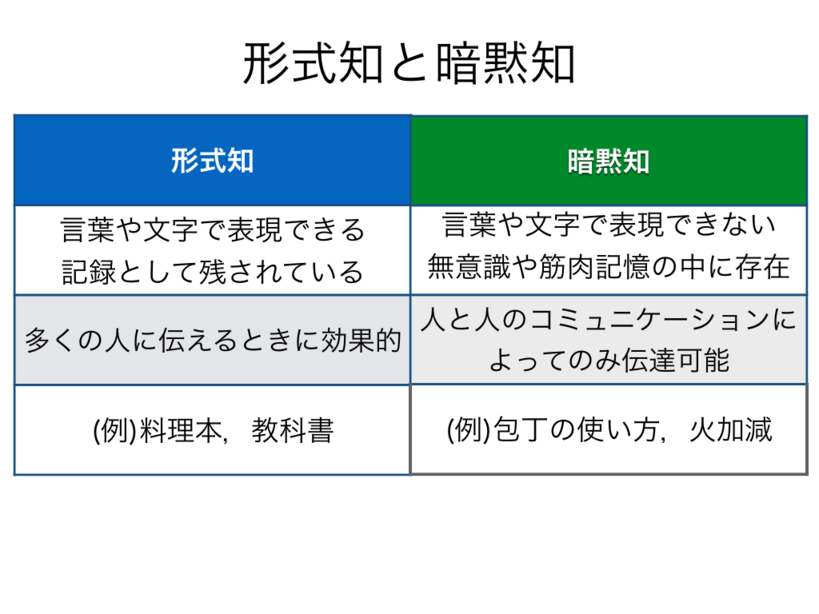
\includegraphics[width=6cm,bb=100 100 600 700]{my_help2hiki_saki.001.png}
\caption{暗黙知と形式知の違い.}
\label{knowledge}\label{default}\end{center}\end{figure}


暗黙知の形式知化はいくつも行われており,google検索したときによく見るQiita.comなどもそれらをまとめるサイトを提供している.
西谷研究室では,各所属学生の暗黙知を形式化するために,my\_helpというgemを開発し,自分のためのメモを残して活用している.
本研究では,西谷研究室内でのナレッジマネジメントを推進するため,
図\ref{my_help2hiki}のようなメモソフトmy\_helpからwiki cloneのhikiへ自動変換するシステムの開発と,
my\_helpをよりよいソフトにするためにFrontPageの設計をする.

\begin{figure}[htbp]
\begin{center}
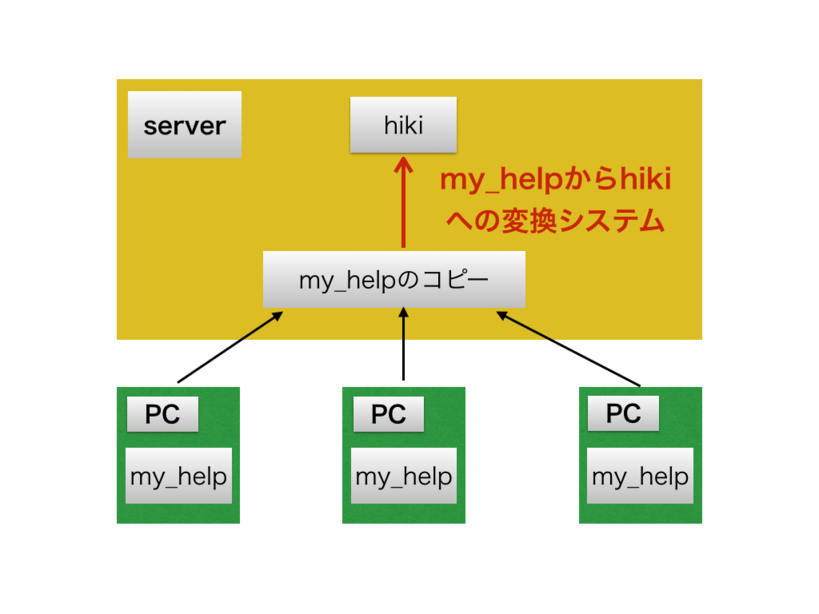
\includegraphics[width=6cm,bb=100 100 600 700]{my_help2hiki_saki.011.png}
\caption{my\_helpからhikiへの自動変換システム.}
\label{my_help2hiki}\label{default}\end{center}\end{figure}

本論文の構成は次の通りである.
対象とするソフトはあまり一般に普及しているものではないため,
最初にソフトの特徴と簡単な振る舞いを紹介する.
次に3章では開発するシステムの使用法を想定し,設計仕様を述べる.
4章では作成したソフトの振る舞いとコードの中身を詳述して,結論をまとめた.
5章では今後これらの変換ソフトを使ってwebを作成するための
プロトタイプを作成し,そこで必要とされる機能について検討を行っている.
6章で今後の課題を記した.

